\begin{center}
  \section{教务系统设计}
\end{center}

\subsection{系统框架}\label{sec:system_frame}
本系统基于层次化、模块化的思想进行搭建和开发。系统分为三层,分别为:表示层,控制层以及实体层。该三层分层结构具有明晰的依赖关系,表示层依赖于控制层,控制层调用实体层,如图\ref{fig:level_depend}所示。本文使用包图的形式描述系统各层各模块的依赖关系,如图\ref{fig:system_arch}所示。

\subsubsection{表示层}
  
表示层是用户与系统交互的界面,负责获取用户的请求和信息,展示系统的操作结果给用户。本系统表示层的模块包括:“登录认证”、“课程管理”、“教学评分”、“成绩管理”和“管理员维护”。
  
\subsubsection{控制层}
  
控制层是系统业务逻辑的核心,控制管理系统的运行。它负责接收用户的请求和信息,调用实体层的数据,执行系统的业务逻辑操作,并最终将操作结果返回给用户。本系统控制层的模块包括:“用户管理”、“课程管理”、“成绩管理”和“教学评分管理”。
  
\subsubsection{实体层}
  
实体层是系统的数据实体层,在实体层与控制层之间是数据访问对象层(DAO),DAO层提供了控制层访问实体层的接口方法。本系统实体层的模块包括:“用户信息”、“课程信息”、“选课信息”和“教学评分信息”。

\begin{figure}[H]
  \centering
  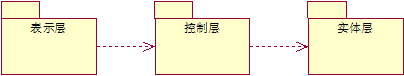
\includegraphics[width=0.8\textwidth]{img/level_depend}
  \caption{层依赖关系}
  \label{fig:level_depend}
\end{figure}

\begin{figure}[H]
  \centering
  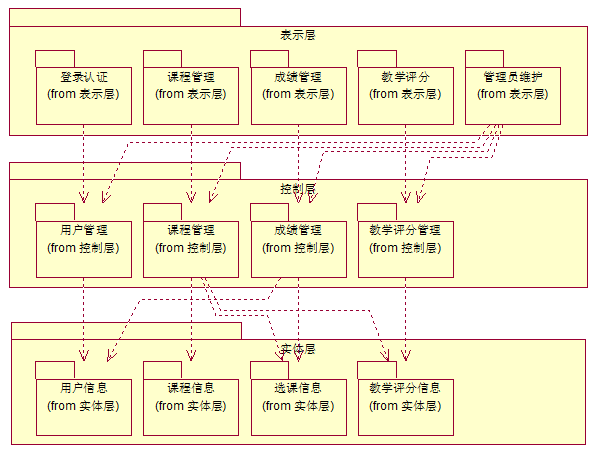
\includegraphics[width=\textwidth]{img/jwxt_system_arch}
  \caption{系统框架图}
  \label{fig:system_arch}
\end{figure}

\subsection{系统关键抽象}\label{sec:system_key_abstract}
系统关键抽象即系统实体类图,系统实体类图描述了系统中的类及其相互之间的关系,它反映了系统中包含的各种对象的类型以及对象间的各种静态关系。图\ref{fig:system_entity}是对实体层中各模块的细化,主要描述了系统实体层中各实体类的属性及其相互的关系。

\begin{figure}[H]
  \centering
  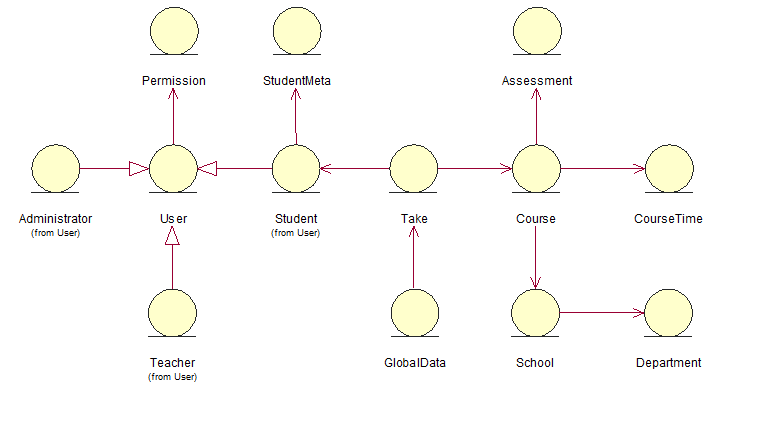
\includegraphics[width=0.95\textwidth]{img/system_entity}
  \caption{系统实体类图}
  \label{fig:system_entity}
\end{figure}
\subsection{用例分析}
\subsubsection{分析类及其功能}
由于系统的用例较多,难以一一列举,所以选取“选课”和“查询成绩”两个用例进行详细分析。其它的用例分析与此两例相似。每个用例分析由四部分组成,第1部分用例功能描述,对用例功能进行简单的描述,第2部分用例交互过程,主要描述了用户与系统的交互工程,采用时序图进行描述,第3部分用例的类分析和实现,描述了用例涉及的各种类,包括边界类,控制类和实体类,第4部分分析类关联关系,描述了分析类的关联关系。

\paragraph{选课用例分析}
\subparagraph{选课用例功能描述}
学生可以利用本功能注册当前学期提供的课程。

\subparagraph{选课用例交互过程}
    
该用例始于学生使用“选课”功能。
    
\begin{enumerate}
  \item 系统从课程目录系统中得到课程类别列表(公必、专必、公选、专选),并将列表显示给学生;
  \item 学生选择课程类别;
  \item 系统从课程目录系统中得到相应课程类别中的课程列表,对列表中的课程检验学生是否满足必要的预备条件,课程是否未被选满且没有时间冲突,然后将满足以上约束的课程列表显示给学生;
  \item 学生从课程列表中选择课程;
  \item 一旦学生决定了选择某门课程,系统将学生添加到该门课程,用该门课程的课程信息更新课程表,并用“已登记”在课程表中对该门课程进行标记。
\end{enumerate}
    
图\ref{fig:selectcourse_secquence}是选课用例的时序图
\begin{figure}[htbp]
  \centering
  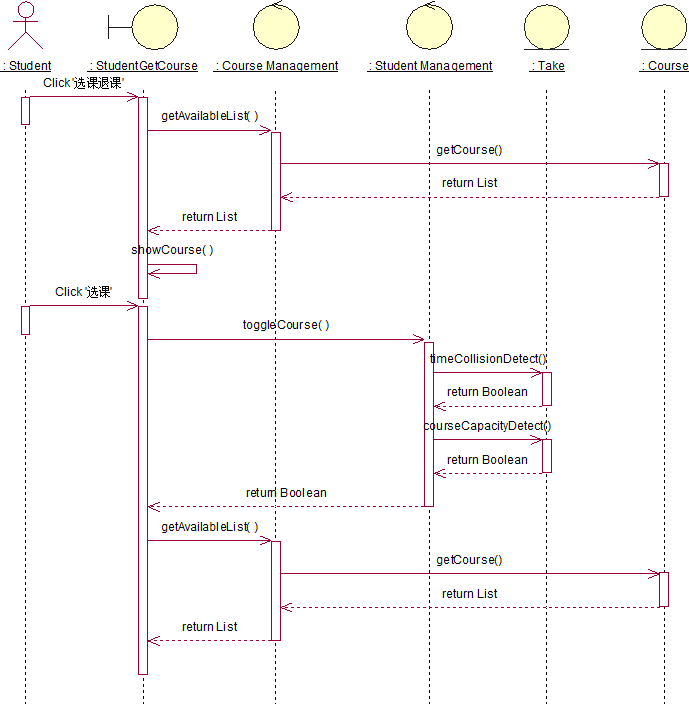
\includegraphics[width=0.7\textwidth]{img/selectcourse_secquence}
  \caption{选课用例时序图}
  \label{fig:selectcourse_secquence}
\end{figure}
    
\subparagraph{选课用例的类分析与设计}
\begin{itemize}
  \item 边界类:课程列表界面(~\texttt{SelectCourse}~)。该界面的组件以表单为主,用于显示该学生本学期可选课程,以及获取学生的选课请求。

  \item 控制类:课程管理(~\texttt{CourseManager}~)。调用~\texttt{getTakes()}~方法获取已选课信息,调用\texttt{getCourses()}获取可选课程信息。获取学生选课请求之后,调用~\texttt{checkCollision()}~\\检测待选课程是否与已选课程存在冲突;若无冲突,则调用~\texttt{take()}~把选课课程加入到选课信息表中;最后再调用~\texttt{getTakes()}~和~\texttt{getCourses()}~更新已选课程列表和可选课程列表。

  \item 实体类:实体类有两个,分别为选课信息(~\texttt{Takes}~)和课程信息(~\texttt{Course}~)。前者存储了学生选课的各种信息,包括选课课程信息、学生信息、课程成绩等;后者存储课程信息,包括课程名、开课院系、老师名、开课时间、学分、考查方式、课程类别、教学评分平均成绩及已进行教学评分的人数等等。
\end{itemize}
    
\subparagraph{选课用例分析类关联关系}
\begin{figure}[H]
  \centering
  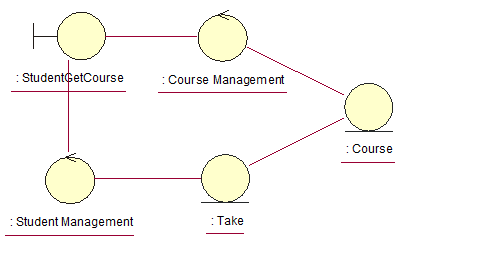
\includegraphics[width=\textwidth]{img/selectcourse_depend}
  \caption{选课用例分析类关联关系图}
\end{figure}
  
\paragraph{查询成绩用例分析}
\subparagraph{查询成绩用例功能描述}

学生可以利用本功能查询个人已选课程的成绩。
    
\subparagraph{查询成绩用例交互过程}
    
该用例始于学生使用“查询成绩”功能。
\begin{enumerate}
  \item 系统检测学生是否完成教学评分,若已完成则显示学年度、学期、培养类别、课程类别、课程名称(可选)的选项,否则跳转到教学评分页面;
  \item 学生选择需查询成绩的学期;
  \item 系统返回相应学期该学生已选课程的课程成绩并显示。
\end{enumerate}
    
图\ref{fig:query_achievement_sequence}是查询成绩用例的时序图
\begin{figure}
  \centering
  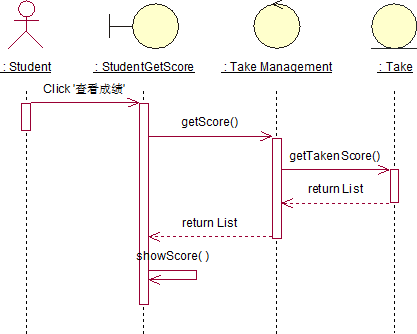
\includegraphics[width=0.7\textwidth]{img/query_achievement_sequence}
  \caption{查询成绩用例时序图}
  \label{fig:query_achievement_sequence}
\end{figure}
    
\subparagraph{查询成绩用例的类分析与设计}
\begin{itemize}
  \item 边界类:查询成绩界面(~\texttt{GetScore}~)。该界面的组件以表单为主,用于获取学生查询某学期成绩的请求,并显示该学生相应学期的课程成绩。
  \item 控制类:成绩管理(~\texttt{ScoreManager}~)。当获取学生查询某学期成绩的请求之后,调用~\texttt{getTakes()}~取得该学生相应学期的选课列表信息。通过该列表的条目,先判断该学生是否完成教学评分。若无,则跳转至教学评分界面;否则提取条目中的成绩信息,并调用~\texttt{getCourses()}~获取该课程名称、学分等信息,最后将这些信息一并显示到查询成绩界面中。
  \item 实体类:实体类有两个,分别为选课信息(~\texttt{Takes}~)和课程信息(~\texttt{Course}~)。前者存储了学生选课的各种信息,包括选课课程信息、学生信息、课程成绩等;后者存储课程信息,包括课程名、开课院系、老师名、开课时间、学分、考查方式、课程类别、教学评分平均成绩及已进行教学评分的人数等等。
\end{itemize}
    
\subparagraph{查询成绩用例分析类关联关系}
\begin{figure}[H]
  \centering
  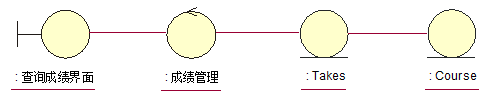
\includegraphics[width=\textwidth]{img/query_achievement_depend}
  \caption{查询成绩用例分析类关联关系图}
\end{figure}

\subsubsection{分析类到分析机制映射}
由于系统的用例较多,难以一一列举分析类到分析机制映射,因此只针对查询成绩用例进行分析类到分析机制映射。涉及的分析类有选课信息类(~\texttt{Takes}~),课程信息类(~\texttt{Course}~),成绩管理类。分析类到分析机制的映射如表\ref{table:anaClass_to_anaMechanism}所示。

\begin{table}[H]
  \caption{部分分析类到分析机制映射表}
  \label{table:anaClass_to_anaMechanism}
  \begin{tabularx}{\textwidth}{|Y|Y|}
  \hline
  \textbf{分析类}&\textbf{分析机制}\\
  \hline
  选课信息&永久性、安全性\\
  \hline
  课程信息&永久性、安全性\\
  \hline
  成绩管理&分布式、安全性\\
  \hline
  \end{tabularx}
\end{table}
\subsubsection{系统类图}
\begin{figure}[htbp]
  \centering
  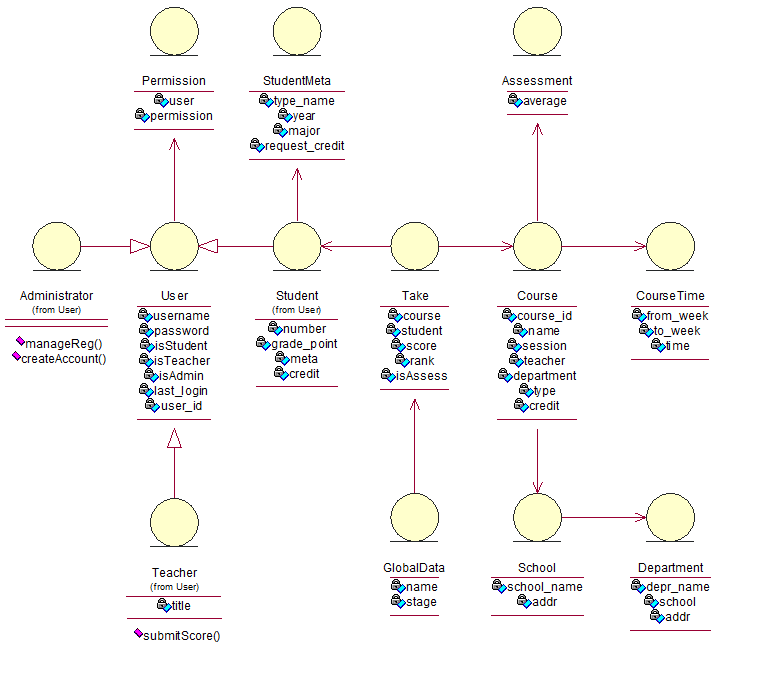
\includegraphics[width=0.95\textwidth]{img/system_class}
  \caption{系统类图}
\end{figure}

\subsection{子系统设计}
本节在\ref{sec:system_frame}系统框架和\ref{sec:system_key_abstract}系统关键抽象的基础上,将系统划分成四个逻辑上相独立,功能上相依赖的子系统(模块),并对用户管理子系统和课程管理子系统进行分析。
\subsubsection{子系统划分}\label{sec:subsystem_div}
本小节在\ref{sec:system_frame}系统框架和\ref{sec:system_key_abstract}系统关键抽象的基础上,将系统划分成四个逻辑上相对独立的子系统(模块),分别为:用户管理子系统,课程管理子系统,成绩管理子系统,教学评分管理子系统。每个子系统(模块)包含了表示层,控制层以及实体层的类,如:在用户管理子系统中,包括了表示层的用户登录界面、注册和注销用户、用户权限管理界面,控制层的输出校验类,实体层的用户类等。\ref{sec:subsystem_design}子系统设计将对用户管理子系统以及课程管理子系统进行详细介绍。
\subsubsection{子系统设计}\label{sec:subsystem_design}
本小节以用户管理子系统和课程管理子系统为例,介绍子系统设计,包括子系统接口,子系统的内部模块划分,各种类以及类的依赖关系。

\begin{figure}[H]
  \centering
  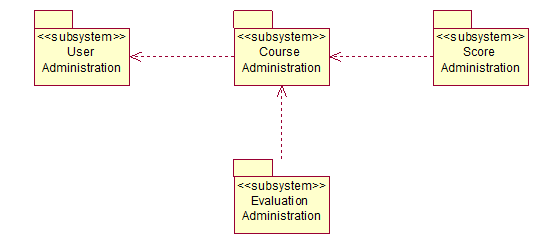
\includegraphics[width=0.8\textwidth]{img/subsystem_depend}
  \caption{子系统依赖图}
  %\label{fig:subsystem_depend}
\end{figure}

\paragraph{用户管理子系统}
  
用户管理子系统实现了用户实体的业务逻辑功能,如:用户登录、注册或注销用户等功能。图\ref{fig:subsystem_usermanage_interface}为用户管理子系统的接口类图。
\begin{figure}[t]
  \centering
  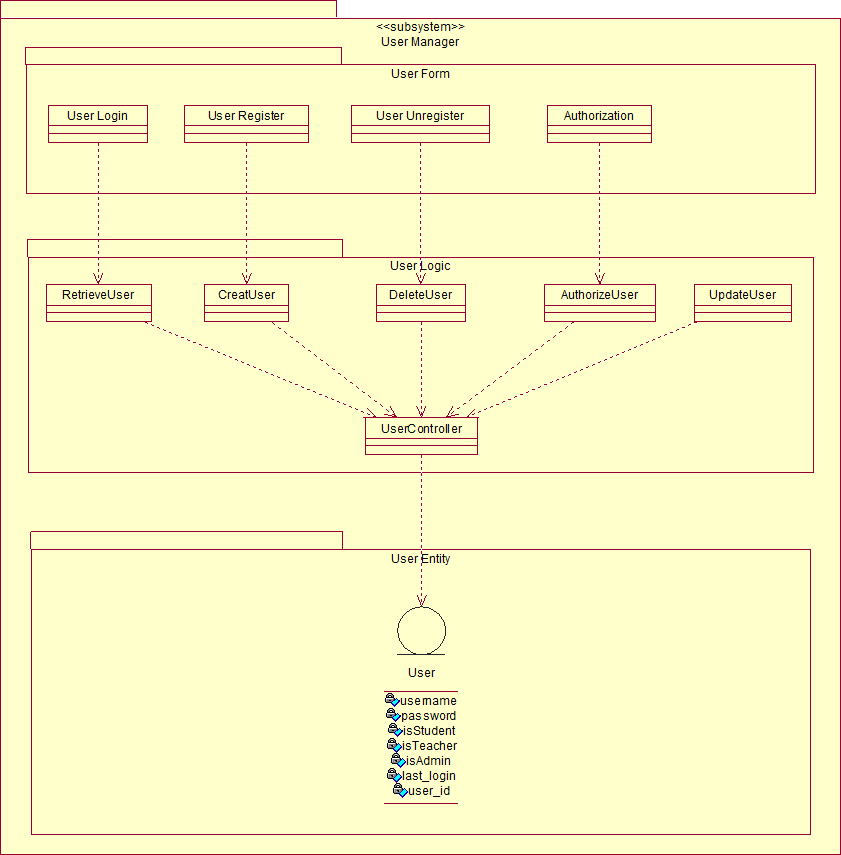
\includegraphics[width=0.8\textwidth]{img/usermgr_interface}
  \caption{用户管理子系统的接口类图}
  \label{fig:subsystem_usermanage_interface}
\end{figure}
  
根据\ref{sec:system_frame}系统架构以及用户实体的业务逻辑功能,可将用户管理子系统分成三个子模块,包括:用户表单,用户管理以及用户实体,分别对应于\ref{sec:system_frame}系统框架的表示层,控制层以及实体层。
  
\begin{itemize}
  \item 用户表单子模块
    
  \CJKindent 对应于\ref{sec:system_frame}系统框架的表示层,该模块主要包含用户表示层的各种表单,如:用户登录表单,用户注册表单,用户注销表单。
    
  \item 用户管理子模块
    
  \CJKindent 对应于\ref{sec:system_frame}系统框架的控制层,该模块主要包含关于用户实体的各种业务逻辑类,如:查找用户,遍历用户等功能。此外,该模块提供了与课程管理子系统、成绩管理子系统及教学评分管理子系统的接口。
    
  \item 用户实体子模块
    
  \CJKindent 对应于\ref{sec:system_frame}系统框架的实体层,该模块包含用户实体类(~\texttt{User}~),实现数据的持久化。
\end{itemize}
  
\paragraph{课程管理子系统}
  
课程管理子系统是教务系统功能的核心,其主要功能是学生选课、退课,学生查询课程信息,教师选择开课课程。图\ref{fig:subsystem_coursemgr_interface}为课程管理子系统的接口类图。
  
\begin{figure}[H]
  \centering
  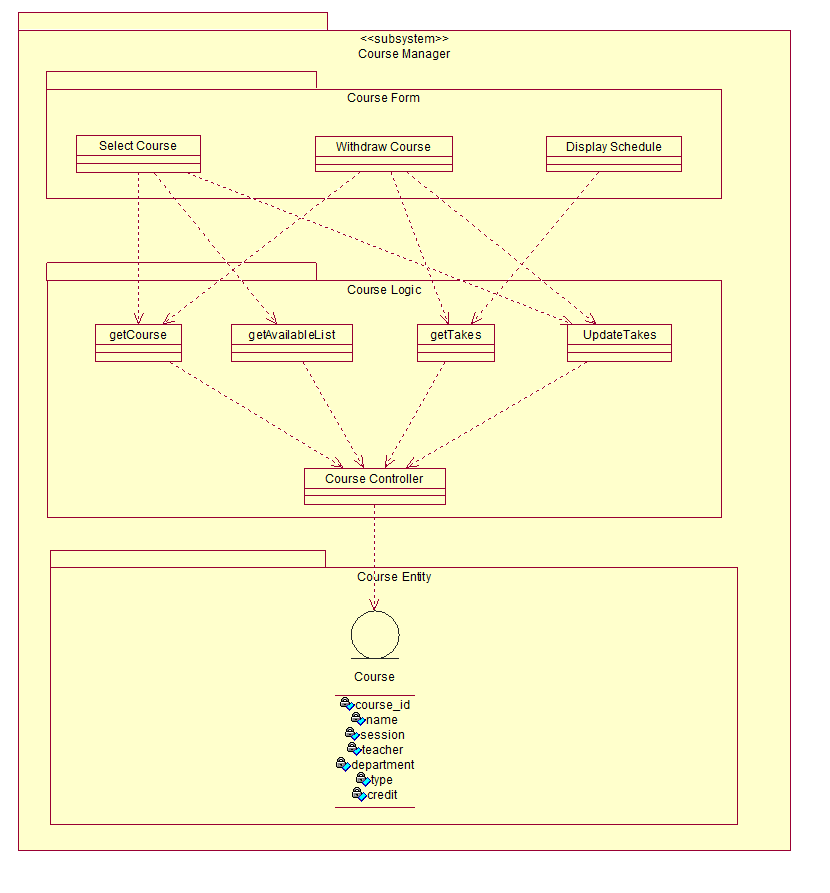
\includegraphics[width=0.8\textwidth]{img/coursemgr_interface}
  \caption{课程管理子系统的接口类图}
  \label{fig:subsystem_coursemgr_interface}
\end{figure}
  
\begin{itemize}
  \item 用户操作子模块
    
  \CJKindent 对应于\ref{sec:system_frame}系统框架的表示层,该模块主要包含括了用户表示层中的课程操作部分,如:显示学生课程表、显示可选课程列表、选课及退课表单、课程详情页面。
    
  \item 课程管理子模块
    
  \CJKindent 对应于\ref{sec:system_frame}系统框架的控制层,该模块主要包含关于课程管理实体的各种业务逻辑类,如:获取已选课表,获取可选课程列表,处理选课及退课请求。

  \item 课程实体子模块
    
  \CJKindent 对应于\ref{sec:system_frame}系统框架的实体层,该模块包含课程实体类(~\texttt{Course}~)和选课信息类(~\texttt{Takes}~),实现数据的持久化。
\end{itemize}

\subsubsection{分析类到设计元素映射}
系统的分析类到设计元素的映射关系如表\ref{table:anaClass_to_designElements}所示。系统的分析类被映射为四个子系统。

\begin{table}[H]
  \caption{分析类到设计元素映射}
  \label{table:anaClass_to_designElements}
  \begin{tabularx}{\textwidth}{|Y|Y|}
  \hline
  \textbf{分析类}&\textbf{设计元素}\\
  \hline
  用户管理功能&用户管理子系统\\
  \hline
  课程管理功能&课程管理子系统\\
  \hline
  成绩管理功能&成绩管理子系统\\
  \hline
  教学评分功能&教学评分管理子系统\\
  \hline
  \end{tabularx}
\end{table}
\subsubsection{设计元素及其包}

由于系统的四个子系统逻辑上相对独立,故将每个子系统设置为一个包,包中包含了实现该子系统的各种类,包括表示类,控制类以及实体类等。子系统包的详细划分可参考\ref{sec:subsystem_div}子系统划分和\ref{sec:subsystem_design}子系统设计。各子系统的分包情况如表\ref{table:designElements_and_package}所示。

\begin{table}[H]
  \caption{设计元素分包情况}
  \label{table:designElements_and_package}
  \begin{tabularx}{\textwidth}{|Y|Y|}
    \hline
    \textbf{设计元素}&\textbf{包}\\
    \hline
    用户管理子系统&用户管理包\\
    \hline
    课程管理子系统&课程管理包\\
    \hline
    成绩管理子系统&成绩管理包\\
    \hline
    教学评分管理子系统&教学评分管理包\\
    \hline
  \end{tabularx}
\end{table}
